% =====================================================================
% Paper 1 — COMFHA
% "Contact without Commitment: Atomistic Characterisation of beta-Lactoglobulin
%  Adsorption Dynamics at the Air-Water Interface"
% Target venue: Journal of Colloid and Interface Science (JCIS)
% Draft v3 — May 28, 2026
% =====================================================================

\documentclass[11pt,a4paper]{article}

\usepackage[utf8]{inputenc}
\usepackage[T1]{fontenc}
\usepackage{lmodern}
\usepackage{microtype}
\usepackage[margin=1in]{geometry}
\usepackage{amsmath,amssymb}
\usepackage{graphicx}
\usepackage{booktabs}
\usepackage{xcolor}
\usepackage{siunitx}
\DeclareSIUnit{\Molar}{M}
\DeclareSIUnit{\angstrom}{\text{\AA}}   % suppress siunitx v3 deprecation warning
\DeclareSIUnit{\bar}{bar}               % suppress siunitx v3 deprecation warning
\usepackage[round,authoryear]{natbib}
\usepackage{setspace}
\usepackage{lineno}
\usepackage{hyperref}
\hypersetup{colorlinks=true, linkcolor=blue!50!black, citecolor=blue!40!black, urlcolor=blue!40!black}
\usepackage[capitalise,noabbrev]{cleveref}

\sisetup{detect-all,per-mode=symbol}
\onehalfspacing
\linenumbers

\bibliographystyle{plainnat}

% ---------------------------------------------------------------------
\title{\large Contact without Commitment: Atomistic Characterisation of
       \boldmath$\beta$-Lactoglobulin Adsorption Dynamics at the Air--Water Interface}

\author{Chalakon Pornjariyawatch \and Prapasiri Pongprayoon\\[2pt]
        \small Department of Chemistry, Faculty of Science,
        Kasetsart University, Bangkok, Thailand\\
        \small Correspondence: chalakon.p@ku.th}

\date{May 2026}
% ---------------------------------------------------------------------

\begin{document}
\maketitle

% =====================================================================
\begin{abstract}
% =====================================================================
\setstretch{1.5}
\noindent
$\beta$-Lactoglobulin (BLG), the most abundant whey protein in bovine milk,
stabilises foam through adsorption at the air--water interface, yet the
molecular mechanism gating this process has remained unresolved. Here we
report the first unbiased atomistic molecular dynamics simulation of BLG
at the air--water interface, using a $12\times12\times35$\,\si{\nano\metre} slab
geometry, the CHARMM36m force field, and TIP3P water across
\SI{4.00}{\micro\second} of cumulative trajectory (one \SI{1000}{\nano\second}
bulk-start run plus three near-interface replicas of
\SI{1000}{\nano\second} each). Resolving adsorption at
single-atom contact distance (rather than centre-of-mass distance, which
is blind to surface contact for a $\sim$\SI{4}{\nano\metre} globular
protein), we find that BLG samples the interface repeatedly under
unbiased dynamics. Across all four trajectories the protein makes
\num{613} discrete contact events --- \num{97} from bulk (\SI{12.5}{\percent}
of frames) and \num{516} from near-interface starts
(\SIrange{7.1}{23.4}{\percent} of frames per replica) --- with single
atoms penetrating up to \SI{0.71}{\nano\metre} past the interface plane.
Only six of these \num{613} events sustain continuous residency
above \SI{10}{\nano\second}, and none commits: the protein
overwhelmingly touches the interface and retreats.
We characterise the pre-commitment contact ensemble: the hydrophobic
calyx is confined to SASA \SIrange{24}{37}{\nano\metre\squared}
throughout (mean \SI{28.95}{\nano\metre\squared}, corrected for
periodic-boundary-condition artefacts), and calyx orientation is
uniformly distributed and statistically independent of SASA:
Pearson $r = +0.006$ (block bootstrap 95\% CI $[-0.09, +0.11]$, block
length \SI{232}{\nano\second} accounting for SASA autocorrelation;
effective $N \approx 17$ independent observations), ruling out linear
coupling at $|r| > 0.11$.
All six long-residency events ($\geq\!\SI{10}{\nano\second}$) are
non-activated contact (event-mean SASA \SIrange{28.5}{30.5}{\nano\metre\squared};
maximum SASA in any event \SI{32.3}{\nano\metre\squared}; zero frames
satisfying SASA $\geq \SI{32.1}{\nano\metre\squared}$ in any event), confirming that
sustained interfacial contact arises without calyx activation. The
protein remains globally compact throughout ($R_\mathrm{g} =
\SI{1.496 \pm 0.009}{\nano\metre}$ in R1; $\beta$-barrel backbone
RMSD \SIrange{0.20}{0.24}{\nano\metre} across all three near-interface
replicas), with loop CD/EF the dominant flexible region near the
interface rather than the global unfolding traditionally invoked to
explain interfacial activity.
These results establish what \SI{4.00}{\micro\second} of unbiased
atomistic MD resolves: the pre-commitment contact ensemble, with its
SASA and orientation distributions, and where the simulation boundary
lies --- gate-open and commitment steps are not sampled on this
timescale, and enhanced sampling is required to characterise the
activation barrier.
\end{abstract}

\vspace{6pt}

\noindent\textbf{Keywords:} $\beta$-lactoglobulin; air--water interface;
molecular dynamics; protein adsorption; contact ensemble; foam stability;
hydrophobic exposure; CHARMM36m.

% =====================================================================
\section{Introduction}
% =====================================================================

The stability of dispersed gas--liquid systems --- foams, whipped emulsions,
aerated dairy products --- is dictated by the proteinaceous film that
assembles at the air--water interface. Adsorbed proteins form a viscoelastic
monolayer that resists film drainage and bubble coalescence, and the molecular
identity of the interfacial protein determines both the rate at which the film
forms and its long-time mechanical
properties\citep{Dickinson1999,BertonCarabin2018,Damodaran2005,Narsimhan2018}. In bovine
milk and its derived ingredients, $\beta$-lactoglobulin (BLG, $\sim$\SI{3}{\gram\per\litre})
is the dominant interfacial protein and the principal stabiliser of milk
foam\citep{Cornec1999,Barbiroli2022,Huppertz2010}. Despite this central technological role,
the question of \emph{how} a folded, water-soluble protein recognises and
populates the air--water interface remains open at the atomic scale.

Experimental tensiometry, ellipsometry, and neutron reflectometry have
established the phenomenology: BLG adsorbs over seconds to minutes, exhibits
a kinetic energy barrier that distinguishes it from more flexible whey
proteins, and partially unfolds in the adsorbed
state\citep{Cornec1999,Mackie1999,Ulaganathan2017a,Ulaganathan2017b,Gochev2019JPCB,Foam4_2020,Perriman2007}. These methods, however,
report time-averaged ensembles rather than the individual conformational
events that actually carry the protein from bulk to interface, and the
classical interpretation --- that adsorption requires global protein
unfolding under interfacial tension\citep{Graham1979} --- has never been
directly observed at atomistic resolution.

Atomistic molecular dynamics offers the complementary lens. To date, however,
MD studies of BLG at fluid interfaces have focused exclusively on
oil--water systems, in which the protein is pre-positioned near the interface
and simulated for tens to hundreds of
nanoseconds\citep{Zare2015,Zare2016}. The air--water interface --- with
surface tension $\sim$\SI{72}{\milli\newton\per\metre} versus
$\sim$\SI{20}{\milli\newton\per\metre} for decane --- is qualitatively
distinct, and no atomistic simulation of BLG at this interface has been
reported. Broader simulations of other proteins at the air--water interface
have targeted hydrophobins\citep{Magarkar2014}, model systems\citep{Euston2010,Cieplak2014},
and orientation-resolved dynamics via MD combined with sum-frequency
spectroscopy\citep{Alamdari2020}, but none has addressed the native fold of
a globular lipocalin starting from bulk solution. Experimentally,
vibrational sum-frequency generation has revealed that BLG orientation
at the air--water interface depends on ionic environment and modulates
adsorption efficiency\citep{Beierlein2015}, implicating patch orientation
as a key variable --- but the molecular origin of this orientation dependence
has not been resolved. The most closely related
study is by Saurabh \textit{et al.} on a monoclonal antibody at the
water/vapour interface over \SI{200}{\nano\second}, but their work employed
thermally pre-stressed conformations rather than the native fold\citep{Saurabh2024}.

Here we present the first unbiased atomistic simulation of native-state BLG
at the air--water interface, totalling \SI{4.00}{\micro\second} of
cumulative trajectory in a $12\times12\times35$\,\si{\nano\metre} slab. We find that
the interfacial dynamics splits cleanly into two physically distinct events
that prior interpretations had conflated: \emph{contact}, in which a
protein heavy atom touches the interface, and \emph{commitment}, in which
the protein remains at the interface long enough to seed a stable
adsorbed state. Resolved at single-atom rather than centre-of-mass
distance, contact is common and rapid; commitment is rare. We characterise the
pre-commitment contact ensemble and establish where the boundary of
unbiased simulation lies: calyx SASA and orientation are statistically
independent coordinates on the \si{\micro\second} timescale, gate-open
and commitment steps are not sampled, and enhanced sampling is required
to resolve the candidate rate-limiting molecular events that explain the
kinetic energy barrier observed experimentally for decades. Specifically,
we contribute:
\begin{enumerate}
  \item the first atomistic MD simulation of BLG at the air--water interface,
        on $\mu$s timescales;
  \item the first atomistic resolution of the contact/commitment
        distinction in protein adsorption: across \SI{4.00}{\micro\second}
        of aggregate trajectory and four independent simulations, the
        protein makes \num{613} discrete contact events
        (\SIrange{7.1}{23.4}{\percent} of frames per trajectory), with
        single atoms penetrating up to \SI{0.71}{\nano\metre} past the
        interface plane; six events sustain residency above
        \SI{10}{\nano\second} (four in R1, one each in CENTER and R3),
        yet none is gate-open or committed --- all are non-activated
        contact (event-mean SASA \SIrange{28.5}{30.5}{\nano\metre\squared},
        zero activation-criterion frames in every event), showing that
        the contact/commitment dichotomy is not bridged by calyx
        activation on the simulated timescale; and
  \item the characterisation of the pre-commitment contact ensemble:
        calyx SASA confined to \SIrange{24}{37}{\nano\metre\squared}
        with orientation uniformly distributed and independent of SASA
        (Pearson $r = +0.006$, block bootstrap 95\% CI $[-0.09, +0.11]$,
        ruling out $|r| > 0.11$ coupling; effective $N \approx 17$
        independent observations after accounting for SASA autocorrelation),
        with loop CD/EF the dominant flexible region near the interface
        rather than the global unfolding traditionally assumed.
\end{enumerate}

% =====================================================================
\section{Results}
% =====================================================================

\subsection{Contact is frequent; commitment is rare}
\label{sec:contact-residency}

We first ran a \SI{1000}{\nano\second} unbiased simulation (SET~1A) with
the BLG monomer placed at the centre of the water slab
($Z \approx \SI{17.5}{\nano\metre}$), equidistant from the upper and lower
air--water interfaces. The protein undergoes diffusive exploration of
the slab, with centre-of-mass $Z$ in the range
\SIrange{15.91}{19.13}{\nano\metre} and a closest centre-of-mass
approach of \SI{1.598}{\nano\metre} at $t = \SI{570}{\nano\second}$.

Centre-of-mass distance, however, is the wrong observable for protein
interfacial contact: BLG has a radius of $\sim$\SI{2}{\nano\metre}, so a
centre-of-mass distance of \SI{1.5}{\nano\metre} already places surface
atoms at or past the interface plane. We therefore measure adsorption by
the minimum distance from any protein heavy atom to the nearest
air--water interface, with a contact threshold of \SI{0.30}{\nano\metre}
(canonical van der Waals contact) and a residency threshold of
\SI{10}{\nano\second} of continuous contact. Under this measure, the
1000 \si{\nano\second} bulk-start trajectory is not silent
(Figure~\ref{fig:fig2}a): protein heavy atoms touch the interface in
\SI{12.5}{\percent} of frames, distributed over \num{97} discrete
contact events, with the deepest single-atom penetration reaching
\SI{-0.474}{\nano\metre} past the interface plane (i.e., the atom
exits the water and is exposed to vacuum) at $t = \SI{570}{\nano\second}$
--- the same physical event the centre-of-mass trace marks as ``closest
approach''. One of these \num{97} events sustains continuous residency above the
\SI{10}{\nano\second} threshold (\SIrange{547.0}{557.5}{\nano\second},
\SI{10.5}{\nano\second}); gate-state analysis confirms this is a
non-activated contact event (hydrophobic SASA below the activation
threshold of \SI{32.1}{\nano\metre\squared} throughout; \cref{sec:gate})
in which non-hydrophobic surface regions remain in contact without gate opening. The remaining \num{96} events terminate
within \SI{10}{\nano\second}: the protein characteristically touches
the interface and retreats.

Three near-interface replicas (SET~1B, R1--R3), each started with the
BLG centre-of-mass \SI{2.183}{\nano\metre} below the upper interface and
extended to \SI{1000}{\nano\second} each, show the same
contact-without-commitment pattern (Figures~\ref{fig:fig2}b and \ref{fig:fig2cd}c--d). R1 makes contact in \SI{23.4}{\percent}
of frames across \num{215} discrete events over \SI{1000}{\nano\second},
with four long-residency windows ($\geq\SI{10}{\nano\second}$) at
\SIrange{362}{419.5}{\nano\second} (\SI{57.5}{\nano\second}),
\SIrange{629.9}{664.4}{\nano\second} (\SI{34.5}{\nano\second}),
\SIrange{665.4}{677.9}{\nano\second} (\SI{12.5}{\nano\second}), and
\SIrange{773.0}{832.0}{\nano\second} (\SI{59.0}{\nano\second}); the
deepest single-atom penetration reaches \SI{-0.71}{\nano\metre} at
$t = \SI{406}{\nano\second}$.
R2 makes contact in \SI{7.1}{\percent} of frames (\num{156} events), with
deepest penetration \SI{-0.52}{\nano\metre} at $t = \SI{864}{\nano\second}$.
R3 makes contact in \SI{10.9}{\percent} of frames (\num{145} events), with
deepest penetration \SI{-0.38}{\nano\metre} at $t = \SI{123}{\nano\second}$.

Across all four trajectories (\SI{4.00}{\micro\second} aggregate), the
\num{613} contact events are overwhelmingly transient: \num{607} terminate
within \SI{10}{\nano\second}. Six events ($\geq\SI{10}{\nano\second}$)
occur across three replicas: one in CENTER (\SI{10.5}{\nano\second}),
four in R1 (\SIrange{12.5}{59.0}{\nano\second}), and one in R3
(\SI{21.8}{\nano\second}). As we show below (\cref{sec:gate}), all six are non-activated contact
events: event-mean SASA ranges from \SI{28.5}{\nano\metre\squared} to
\SI{30.5}{\nano\metre\squared} and zero frames in any event satisfy an
activation criterion. The rarity of commitment --- six long-residency
events in \SI{4.00}{\micro\second}, none committed --- is the central
empirical finding; the contact-ensemble characterisation in \cref{sec:gate}
establishes that gate-open and commitment steps are not sampled on the
microsecond timescale.

The contrast between contact frequency and residency rarity is the
central empirical observation of this work. Adsorption of BLG at the
air--water interface is not limited by the protein's ability to find
the interface (it arrives often, on a sub-microsecond timescale even
from bulk); it is limited by the molecular conditions that determine
whether a contact event commits to stable residency. This empirical
dichotomy reframes the kinetic energy barrier inferred from
experimental adsorption kinetics\citep{Cornec1999,Gochev2019JPCB} from
a transport problem to a residency problem, and motivates the
mechanistic dissection presented in \cref{sec:activation,sec:gate}.

The hydrophobic calyx SASA during the bulk trajectory averages
\SI{28.93}{\nano\metre\squared} (max \SI{36.6}{\nano\metre\squared};
PBC-corrected) and exhibits recurring fluctuations throughout ---
calyx exposure is a stationary stochastic process, not a
pre-adsorption one-shot event. The characterisation of calyx SASA
and orientation during the near-interface trajectories is taken up
in \cref{sec:gate}.

\begin{figure}[tbp]
  \centering
  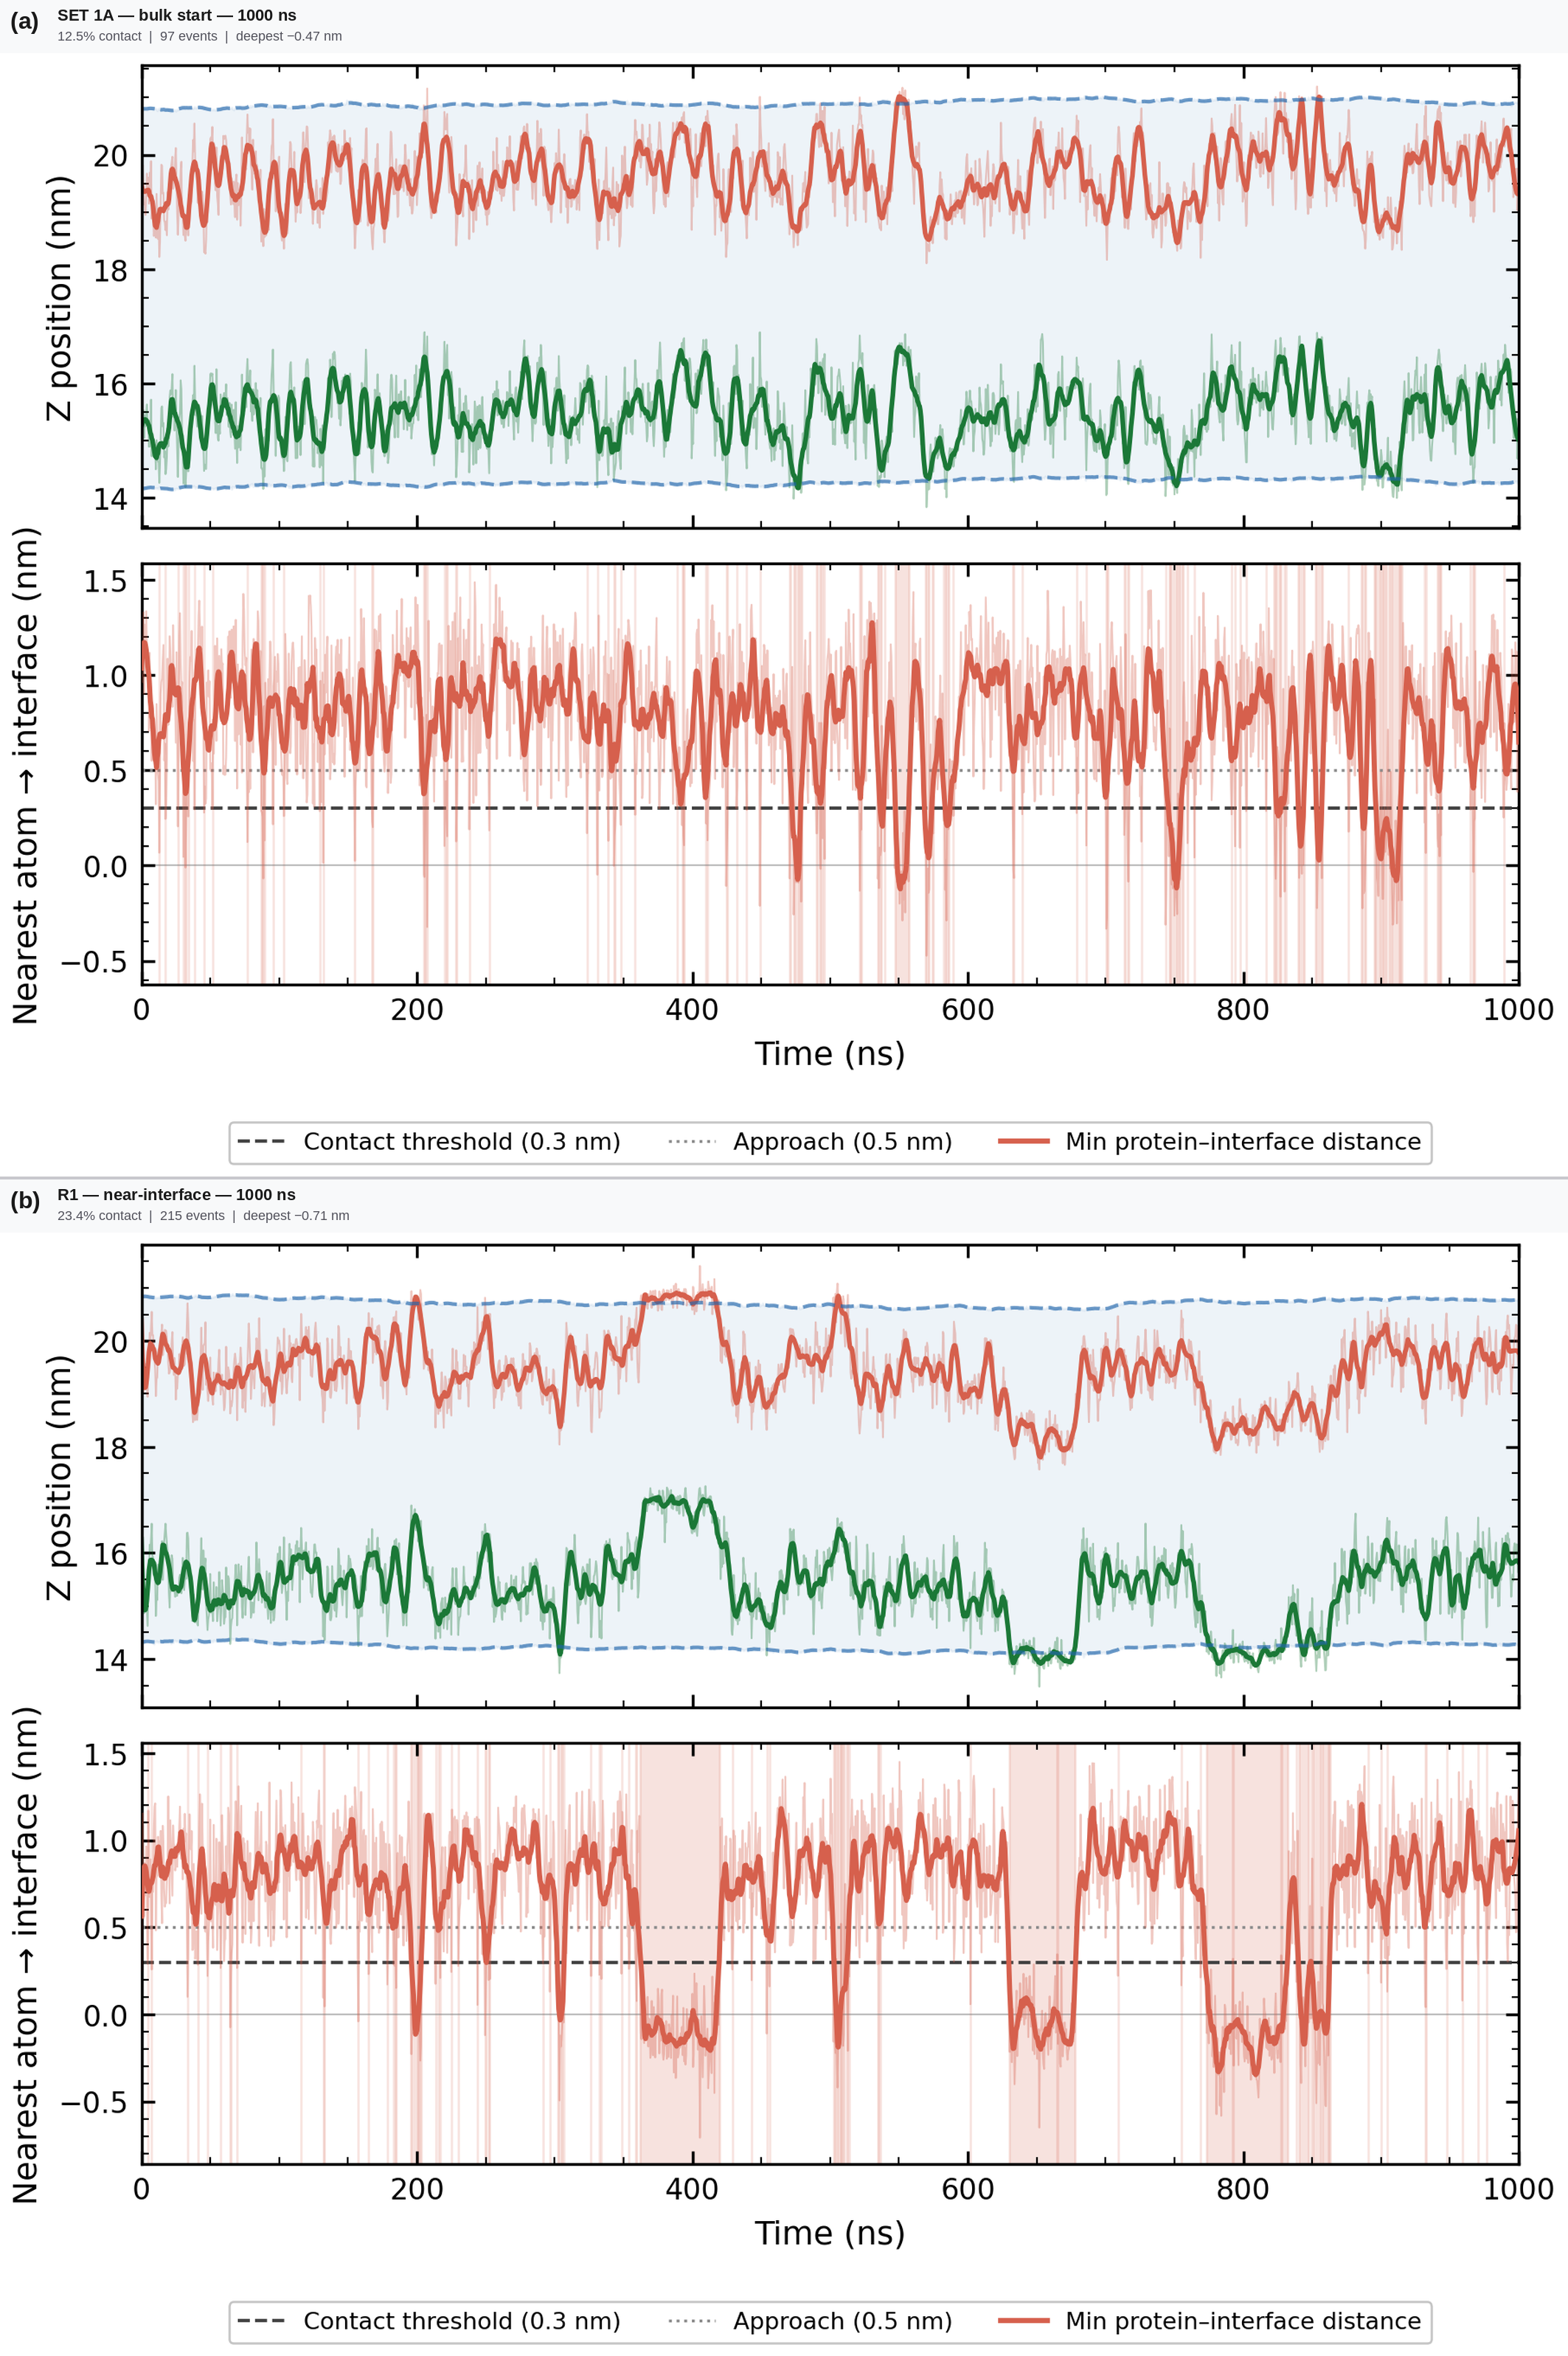
\includegraphics[width=0.88\textwidth,height=0.68\textheight,keepaspectratio]{../../results/figures/PAPER_FIG2_CONTACT_AB.png}
  \caption{\textbf{BLG samples the air--water interface repeatedly but
    rarely commits to stable residency (SET~1A and R1).}
    Single-atom contact analysis: (\textbf{a}) bulk-start trajectory
    (SET~1A, \SI{1000}{\nano\second}); (\textbf{b})~R1
    (\SI{1000}{\nano\second}). In each panel: upper plot shows the
    topmost and bottommost protein heavy-atom $Z$ overlaid on the upper
    and lower air--water interface positions; lower plot shows the
    minimum protein--interface distance, with contact threshold
    \SI{0.30}{\nano\metre} (dashed) and approach threshold
    \SI{0.50}{\nano\metre} (dotted). Shaded bands mark contiguous
    contact windows. Contact fractions: SET~1A \SI{12.5}{\percent}
    (\num{97} events), R1 \SI{23.4}{\percent} (\num{215} events).
    Deepest penetrations: SET~1A \SI{-0.47}{\nano\metre}, R1
    \SI{-0.71}{\nano\metre}. (Continued in \cref{fig:fig2cd}.)}
  \label{fig:fig2}
\end{figure}

\begin{figure}[tbp]
  \centering
  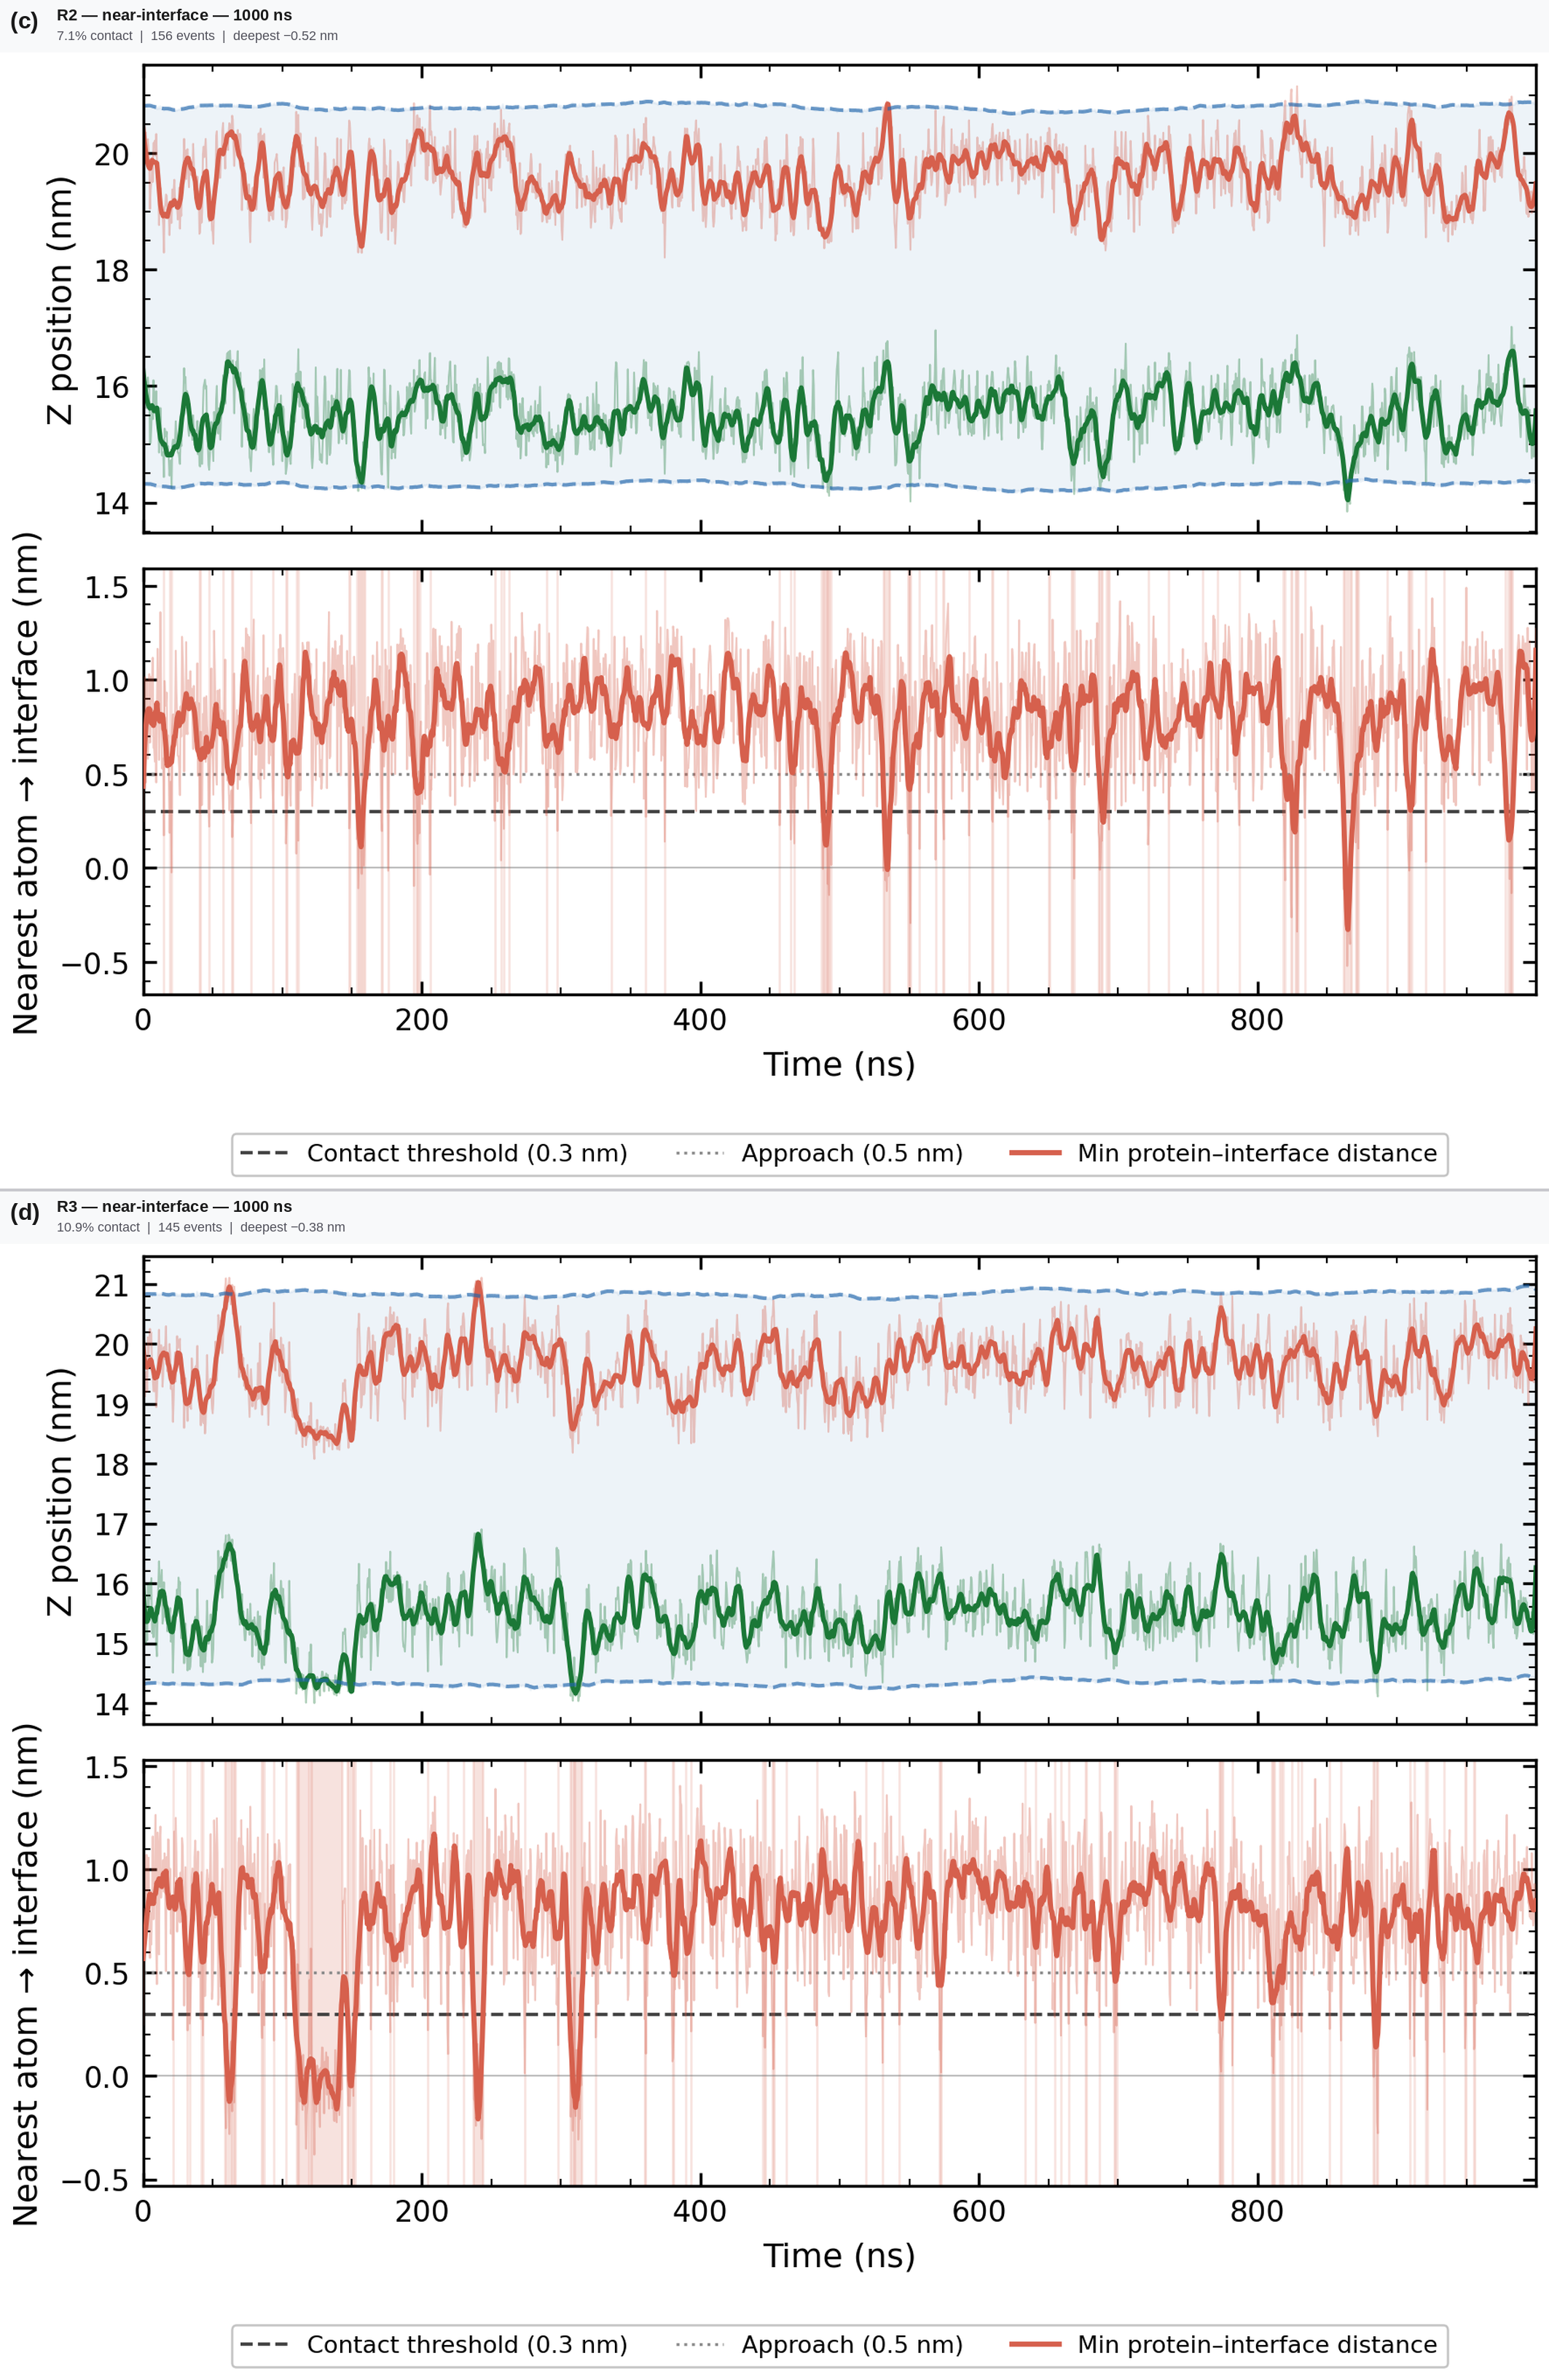
\includegraphics[width=0.88\textwidth,height=0.68\textheight,keepaspectratio]{../../results/figures/PAPER_FIG2_CONTACT_CD.png}
  \caption{\textbf{BLG contact analysis continued (R2 and R3).}
    (\textbf{c})~R2 (\SI{1000}{\nano\second}); (\textbf{d})~R3
    (\SI{1000}{\nano\second}). Same conventions as \cref{fig:fig2}.
    Contact fractions: R2 \SI{7.1}{\percent} (\num{156} events), R3
    \SI{10.9}{\percent} (\num{145} events). Deepest penetrations: R2
    \SI{-0.52}{\nano\metre}, R3 \SI{-0.38}{\nano\metre}. Across all
    \num{613} events aggregate (\cref{fig:fig2,fig:fig2cd}), six
    contact episodes exceed \SI{10}{\nano\second} (one in CENTER, four
    in R1, one in R3; gate-state analysis in \cref{sec:gate} confirms
    all are non-activated contact; \cref{sec:gate}); \num{607} of \num{613} events terminate within
    \SI{10}{\nano\second}. Centre-of-mass distance never falls below
    \SI{1.35}{\nano\metre} --- a metric blind to surface contact for a
    $\sim$\SI{4}{\nano\metre} globular protein.}
  \label{fig:fig2cd}
\end{figure}

\subsection{Calyx dynamics are loop-mediated: compact protein, mobile calyx}
\label{sec:activation}

Having established that contact is frequent but commitment is rare, we
turn to the conformational dynamics of the calyx using the three
near-interface replicas (R1--R3) introduced in \cref{sec:contact-residency}.
The replicas reveal four structural features (Figure~\ref{fig:fig3}). First,
the protein is globally compact throughout: radius of gyration
$R_\mathrm{g} = \SI{1.496 \pm 0.009}{\nano\metre}$ (R1), with no monotonic
trend toward expansion. The alpha-helix (residues 130--142) remains
structurally intact throughout (RMSD $\leq \SI{0.137}{\nano\metre}$ across
all replicas), and the $\beta$-barrel core --- which one might expect to
unravel in preparation for interfacial insertion --- remains assembled
(backbone RMSD \SI{0.218}{\nano\metre} R1, \SI{0.195}{\nano\metre} R2,
\SI{0.238}{\nano\metre} R3). \emph{Under unbiased dynamics (\SI{4.00}{\micro\second}), the protein
never globally unfolds in preparation for adsorption.}

Second, despite this global compactness, the hydrophobic calyx is mobile
throughout. R1 exhibits recurring SASA fluctuations with a characteristic
spacing of \SIrange{30}{40}{\nano\second} (PBC-corrected; SASA range
\SIrange{24}{37}{\nano\metre\squared}): calyx exposure is not a one-shot
pre-adsorption event but a stationary stochastic process.

Third, per-residue RMSF reveals a striking interface-induced shift in which
loop dominates this flexibility. In the bulk SET~1A simulation, Loop~BC
(residues 30--35) is the most flexible region (RMSF max \SI{0.54}{\nano\metre};
Loop~CD/EF max \SI{0.31}{\nano\metre}).
In the near-interface replica R1, this hierarchy inverts: Loop~CD/EF
(residues 57--60) rises to RMSF max \SI{0.39}{\nano\metre} and becomes
the dominant flexible region, while Loop~BC falls to \SI{0.25}{\nano\metre}.
Loop~CD/EF lies directly above the hydrophobic calyx. This quantitative shift indicates an
\emph{interface-induced conformational preference}: proximity to the air--water
interface selects calyx-opening motions over the bulk-default Loop~BC mobility.
Notably, protonation of Glu89 --- which occurs near physiological pH --- also
triggers Loop~CD/EF reorganisation in BLG\citep{Eberini2004}, suggesting
this loop is intrinsically primed for dynamic responses.

Fourth, the hydrophobic patch C$\alpha$ RMSD stays low and bounded
throughout: approximately \SI{0.24}{\nano\metre} at \SI{500}{\nano\second}
and \SI{0.23}{\nano\metre} at \SI{650}{\nano\second} (R1), with no
monotonic upward trend over \SI{1000}{\nano\second}. The calyx residues
explore a structurally defined neighbourhood rather than progressively
opening; the recurring SASA fluctuations are driven by transient loop
motions rather than sustained structural drift of the patch.

Taken together, these four observations support a picture in which
adsorption activation is \emph{loop-mediated} and \emph{calyx-localised},
not the cooperative global unfolding traditionally invoked to explain
protein interfacial activity\citep{Graham1979}.

\begin{figure}[htbp]
  \centering
  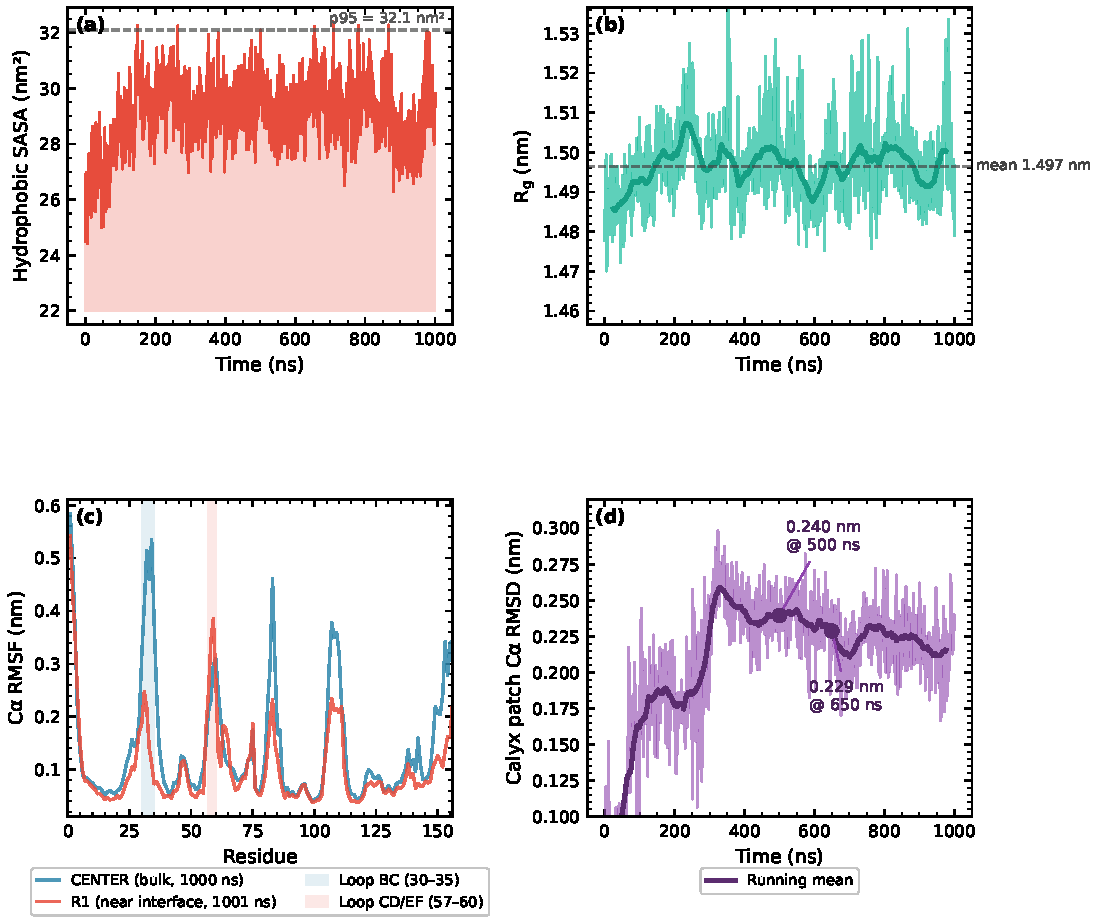
\includegraphics[width=0.95\textwidth]{../../results/figures/PAPER_FIG3_ACTIVATION.pdf}
  \caption{\textbf{Activation is loop-mediated and calyx-localised; the global fold is preserved.}
    Replica~1, full \SI{1000}{\nano\second} trajectory.
    (\textbf{a}) Hydrophobic SASA: recurring fluctuations spanning
    \SIrange{24}{37}{\nano\metre\squared} (PBC-corrected);
    dashed line marks the distribution-based 95th-percentile threshold
    (p95 = \SI{32.1}{\nano\metre\squared}).
    (\textbf{b}) Radius of gyration: mean
    $R_\mathrm{g} = \SI{1.496 \pm 0.009}{\nano\metre}$, no monotonic
    expansion --- under unbiased dynamics, the protein never globally unfolds in
    preparation for adsorption.
    (\textbf{c}) Per-residue C$\alpha$ RMSF for CENTER (blue) and R1 (red).
    In bulk the dominant flexible peak is Loop~BC (residues 30--35,
    blue shading); near the interface the loop CD/EF region
    (residues 57--60, red shading), directly above the hydrophobic
    calyx, becomes structurally relevant --- an interface-induced
    conformational preference.
    (\textbf{d}) Hydrophobic patch C$\alpha$ RMSD remains bounded
    below \SI{0.30}{\nano\metre} throughout (running mean, purple);
    mean $\approx$\SI{0.21}{\nano\metre}, no monotonic trend,
    indicating the calyx samples a structurally defined region rather
    than undergoing progressive opening.}
  \label{fig:fig3}
\end{figure}

\subsection{Calyx exposure and orientation during contact: distribution and independence}
\label{sec:gate}

The two preceding observations stand in tension. The protein makes
heavy-atom contact with the interface in
\SIrange{7.1}{23.4}{\percent} of frames per trajectory
(\num{613} events aggregate, \cref{sec:contact-residency}), and the
hydrophobic calyx is mobile throughout the trajectory
(\cref{sec:activation}). If contact frequency and hydrophobic
exposure were jointly sufficient for adsorption, the protein should
already be adsorbed many times over; yet \num{607} of \num{613} contact
events terminate within the \SI{10}{\nano\second} residency threshold,
and none of the six that exceed it results in commitment.
\emph{Contact does not commit.}

To characterise the pre-commitment contact ensemble we quantify two
coordinates: the hydrophobic calyx SASA and the calyx orientation angle
$\theta$ (between the centre-of-mass-to-calyx-centroid vector and the
$-Z$ axis pointing toward the upper interface). Pooled across all four
PBC-corrected trajectories (\num{8006} frames at
\SI{0.5}{\nano\second} stride), the calyx SASA spans
\SIrange{23.4}{36.7}{\nano\metre\squared} with mean
\SI{28.95}{\nano\metre\squared} (s.d.\ \SI{1.97}{\nano\metre\squared})
--- a compact distribution that does not reach a distinct
``activated'' regime. The calyx orientation is broadly distributed
(mean $94^\circ$, s.d.\ $40^\circ$, spanning \SIrange{1}{179}{\degree}), consistent
with near-isotropic tumbling rather than preferential alignment toward
the interface (Figure~\ref{fig:fig4}).

Critically, the two coordinates are statistically independent. The
Pearson correlation coefficient between SASA and $\theta$, computed
on PBC-corrected data, is $r = +0.006$ (10\,000-resample block
bootstrap 95\% CI $[-0.09, +0.11]$; block length \SI{232}{\nano\second}
estimated from the SASA autocorrelation time; effective $N \approx 17$
independent trajectory segments across 8006 sampled frames), ruling
out linear coupling at $|r| > 0.11$. The large autocorrelation time
reflects the slow fluctuation of the calyx SASA on the hundreds-of-nanosecond
timescale, consistent with the recurring \SIrange{30}{40}{\nano\second}
burst structure visible in Figure~\ref{fig:fig3}a. A previously
reported value of $r = -0.085$ was computed on PBC-artefact-corrupted
SASA data (which inflated SASA up to $\sim$\SI{70}{\nano\metre\squared})
and is superseded by this corrected result.
Consistent with the absence of nonlinear threshold coupling, contingency
analysis across SASA cutoffs from \SIrange{27}{33}{\nano\metre\squared}
yields observed-to-independent ratios (Obs/Indep) in the range 0.87--1.16,
clustering around unity and showing no systematic suppression or
enhancement at any cutoff.

\begin{figure}[htbp]
  \centering
  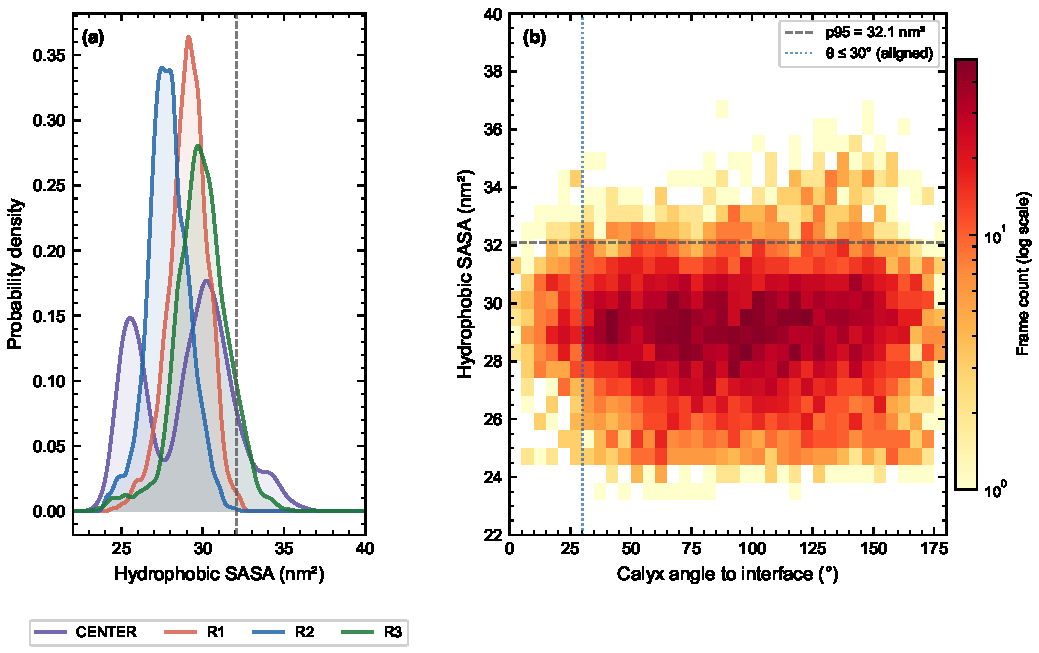
\includegraphics[width=0.95\textwidth]{../../results/figures/Fig4_optionA.pdf}
  \caption{\textbf{Pre-commitment contact ensemble of BLG at the
    air--water interface (all four replicas, PBC-corrected).}
    (\textbf{a}) Calyx SASA distribution per replica (kernel density
    estimate). SASA is confined to \SIrange{24}{37}{\nano\metre\squared}
    across \SI{4.00}{\micro\second} of aggregate trajectory; the
    distribution-based 95th-percentile threshold (p95 =
    \SI{32.1}{\nano\metre\squared}, dashed line) marks the upper tail
    rather than a discrete activated regime. Mean SASA:
    \SI{28.95}{\nano\metre\squared}. (\textbf{b}) Two-dimensional
    joint distribution of calyx orientation angle $\theta$ and SASA
    (all replicas, \num{8006} frames). The distribution is broad and
    structureless: orientation is uniform across the orientation sphere
    and independent of SASA ($r = +0.006$, block bootstrap 95\% CI
    $[-0.09, +0.11]$, ruling out $|r| > 0.11$). The dashed horizontal line marks p95 = \SI{32.1}{\nano\metre\squared};
    the dotted vertical line marks $\theta = 30^\circ$ (shown for
    visual reference; no distinct activated regime was observed to
    be reached, so no specific activation threshold is applied).
    The density is low and diffuse in the high-SASA, low-$\theta$
    corner, reflecting the sparseness of the joint tail rather than
    suppression of a coupled state. At the p95 cutoff: \SI{5.0}{\percent}
    of frames have SASA $\geq$ p95; \SI{5.2}{\percent} have $\theta \leq 30^\circ$;
    Obs/Indep $= 0.92$ (95\% CI 0.54--1.31), consistent with independence.}
  \label{fig:fig4}
\end{figure}

The six $\geq\!\SI{10}{\nano\second}$ residency events provide a direct
view of the long-contact regime (Table~\ref{tab:long-events}). All six
are non-activated contact: event-mean SASA ranges from
\SI{28.5}{\nano\metre\squared} (R3 120.6--142.4\,ns) to
\SI{30.5}{\nano\metre\squared} (CENTER 547--557.5\,ns), and maximum
SASA in any event is \SI{32.3}{\nano\metre\squared} --- well below any
reasonable activation criterion. Zero frames in any event satisfy
$\mathrm{SASA} \geq \SI{35}{\nano\metre\squared}$.

\begin{table}[ht]
  \centering
  \caption{\textbf{Per-event SASA and orientation statistics for the
    six $\geq\!\SI{10}{\nano\second}$ residency events (PBC-corrected).}
    All events are in the non-activated contact regime. Zero frames in
    any event satisfy $\mathrm{SASA} \geq \SI{35}{\nano\metre\squared}$.}
  \label{tab:long-events}
  \begin{tabular}{llrrrr}
    \toprule
    Replica & Window (ns) & $N$ & SASA\textsubscript{mean} (nm$^2$) & SASA\textsubscript{max} (nm$^2$) & $\theta_\mathrm{mean}$ ($^\circ$) \\
    \midrule
    R1      & 362.0--419.5   & 116 & 29.31 & 32.01 &  38.7 \\
    R1      & 629.9--664.4   &  70 & 29.97 & 32.23 & 145.4 \\
    R1      & 665.4--677.9   &  26 & 29.69 & 31.24 & 143.7 \\
    R3      & 120.6--142.4   &  43 & 28.54 & 29.87 &  55.6 \\
    CENTER  & 547.0--557.5   &  22 & 30.47 & 31.81 & 139.3 \\
    R1      & 773.0--832.0   & 119 & 29.77 & 32.26 & 150.8 \\
    \bottomrule
  \end{tabular}
\end{table}

The orientation is diverse across the six events --- ranging from
$\theta_\mathrm{mean} = 38.7^\circ$ (calyx tilted toward the interface)
to $150.8^\circ$ (calyx pointing away) --- indicating that long residency
is geometrically promiscuous and does not require a specific calyx
orientation. This is consistent with the global independence ($r = +0.006$)
found in the full dataset.

These results establish what \SI{4.00}{\micro\second} of unbiased atomistic
MD resolves: the pre-commitment contact ensemble, its SASA and
orientation distributions, and where the simulation boundary lies. The
protein arrives at the interface readily, makes contact often, and
retreats most of the time. The calyx is not detectably more exposed or
more oriented during long-residency events than during the broader
contact ensemble; the molecular step that converts contact to commitment
is not sampled on the microsecond timescale.

% =====================================================================
\section{Discussion}
% =====================================================================

The central finding of this work is an atomistic characterisation of
what the pre-commitment contact ensemble of native BLG at the air--water
interface looks like, and a precise statement of where the boundary of
unbiased \si{\micro\second} MD lies. We resolve a long-standing tension
in the literature: BLG is manifestly surface-active --- it stabilises
foams under physiological conditions --- and yet it adsorbs slowly, with
a kinetic energy barrier\citep{Cornec1999}. The protein makes contact
with the interface frequently (\num{613} events across
\SI{4.00}{\micro\second}), yet \num{607} of those events terminate
within \SI{10}{\nano\second} and none commits. The calyx SASA and
orientation are statistically independent under unbiased dynamics
($r = +0.006$, block bootstrap 95\% CI $[-0.09, +0.11]$), and no gate-open or commitment transition
is observed on the microsecond timescale. The molecular step that
converts contact to commitment lies beyond the accessible timescale of
unbiased MD and requires enhanced sampling to resolve.

The scientific importance of characterising this pre-commitment state
has been underappreciated. Prior classical and coarse-grained adsorption
models typically assumed that any contact event at the interface is
either immediately followed by unfolding and adsorption (e.g., the
surface-denaturation picture\citep{Graham1979}) or is too brief to
matter at all. Neither assumption holds here. The pre-commitment
ensemble is not a fleeting artefact: six contact events exceed
\SI{10}{\nano\second} in duration, one of which lasts \SI{59}{\nano\second},
yet none progresses to commitment. The contact/commitment dichotomy is
therefore a genuine kinetic bottleneck, not a sampling limitation.
The pre-commitment state is characterised by a well-defined SASA and
orientation distribution ($r = +0.006$; Obs/Indep clustering around
unity across all SASA cutoffs), ruling out simple two-factor coupling
as the commitment trigger. This baseline is a prerequisite for
designing enhanced-sampling calculations that correctly define the
reaction coordinate connecting contact to commitment.

This reframing differs sharply from the classical view of Graham and
Phillips, in which interfacial proteins adsorb after surface tension
induces global unfolding\citep{Graham1979}. Our data are inconsistent
with that picture for BLG: the protein remains globally compact
($R_\mathrm{g}$ stable to within \SI{0.6}{\percent} across
\SI{4.00}{\micro\second} of aggregate trajectory), the alpha-helix retains its native fold, and the
$\beta$-barrel scaffold remains assembled throughout the pre-adsorption
regime. Activation is loop-mediated and calyx-localised, not global (as
evidenced by the dominant flexibility of Loop~CD/EF near the
interface relative to Loop~BC in bulk; \cref{sec:activation}). The
notion of ``surface unfolding'' may yet apply to the post-adsorption
state, but the candidate rate-limiting molecular event en route to adsorption is
not global unfolding --- it is a step that lies beyond the reach of
unbiased microsecond MD, most likely requiring a specific coupling of
calyx exposure and orientation that is not sampled on this timescale.

Our contact-ensemble characterisation also contextualises the study by
Saurabh \textit{et al.}\citep{Saurabh2024} on monoclonal antibody
adsorption at the water/vapour interface. Their starting structures were
thermally pre-stressed, bypassing the contact regime characterised here
and starting in a conformationally perturbed state that native-state BLG
does not visit under unbiased dynamics. The contrast in starting
conditions means the two studies probe different parts of the adsorption
pathway.

The contact-ensemble picture has implications for protein engineering of
foam stabilisers. Loop CD/EF (residues 57--60), which becomes the dominant
flexible region near the interface in our simulations, couples calyx
mobility to overall protein dynamics. If commitment requires calyx-face
contact with the interface --- the natural hypothesis given the role of
the hydrophobic patch --- then mutations that increase calyx flexibility
or exposure at the interface may accelerate commitment more effectively
than mutations that merely increase average bulk hydrophobicity. More
broadly, the observation that calyx SASA and orientation are
statistically independent in native-state BLG provides a quantitative
baseline for comparing mutants and variants across the lipocalin
family\citep{Flower1996,Papiz1986}.

This study has several limitations. First, of the \num{613} contact
events observed across \SI{4.00}{\micro\second} of aggregate trajectory,
only six cross the \SI{10}{\nano\second} residency threshold, and all
six are in the non-activated contact regime (SASA
\SIrange{28.5}{30.5}{\nano\metre\squared}; Table~\ref{tab:long-events}).
No contact in any replica grows into an irreversibly adsorbed monolayer
on the experimentally relevant seconds-to-minutes
timescale\citep{Cornec1999,Gochev2019JPCB,Foam4_2020}. The contact/commitment
dichotomy is established empirically, but the molecular mechanism of
commitment --- the step that converts a contact event into an irreversibly
adsorbed state --- is not sampled and cannot be characterised from
unbiased MD alone; protein adsorption from bulk to an irreversibly
adsorbed monolayer encompasses structural rearrangements and cooperative
processes that unfold on timescales from seconds to hours\citep{Rabe2011}.
Resolving the commitment mechanism will require enhanced sampling along
appropriate collective coordinates, such as metadynamics or umbrella
sampling along $(\mathrm{SASA},\,\theta)$.

Second, we simulate the BLG monomer rather than the native dimer, which
is the dominant form at neutral pH and concentrations above
$\sim$\SI{50}{\micro\Molar}\citep{Mercadante2012} --- i.e., over
essentially the entire range in milk and most food-relevant systems
($\sim$\SI{0.16}{\milli\Molar} in bovine milk). The monomer is the
natural starting point for resolving single-molecule mechanism but
dimerisation introduces additional complexity across multiple aspects of
the contact ensemble. Sterically, the dimer interface occludes the
calyx-adjacent Loop~CD/EF region, which we identify here as the dominant
flexible region near the interface; a dimer partner would constrain this
loop's interface-induced mobility and could shift the SASA$_{12}$
distribution toward lower values. Kinetically, the dimer must dissociate
before a monomer can present the calyx face unobstructed at the interface,
adding a dissociation step that is absent in our monomer simulations.
Orientationally, the second monomer doubles the molecular mass and
changes the hydrodynamic shape from roughly spherical to oblate, which
would alter the rotational diffusion and thus the distribution of $\theta$
during contact. In aggregate, the monomer contact ensemble characterised
here represents the most accessible molecular hypothesis --- the behaviour
of an individual lipocalin unit --- but the transition to a dimer-relevant
description is an explicit priority in the next phase of this programme.

Third, the TIP3P water model underestimates the air--water surface
tension by roughly one-third relative to TIP4P/2005 and to
experiment\citep{Vega2007}; we expect this to shift the quantitative
contact and residency statistics rather than qualitatively alter the
contact-ensemble characterisation, but a TIP4P/2005 cross-check on the
SET~1A geometry is a natural follow-up. Fourth, we use a single force
field (CHARMM36m); replication in a non-CHARMM force field (e.g.,
AMBER99SB) is a standard robustness check we have not yet performed.
Fifth, our analysis characterises the contact ensemble under unbiased
dynamics rather than computing free-energy barriers; the activation
free energy along $(\mathrm{SASA},\,\theta)$ or other commitment
coordinates would require metadynamics\citep{Laio2002} or umbrella
sampling and lies outside the scope of this study. Sixth, fat-soluble components and the
second whey protein $\beta$-casein, both relevant in real milk systems,
are addressed in subsequent phases of this study.

% =====================================================================
\section*{Methods}
% =====================================================================
\addcontentsline{toc}{section}{Methods}

\subsection*{Protein structure and force field}

The crystal structure of bovine $\beta$-lactoglobulin was obtained from
the Protein Data Bank (PDB ID: 1BEB, resolution \SI{1.8}{\angstrom},
chain~A)\citep{Brownlow1997,Kontopidis2004}. The hydrophobic calyx is
the defining lipocalin feature of BLG, normally enclosing fatty acids
and other small hydrophobic ligands\citep{Loch2013}. Crystallographic waters and ligands were
removed. The structure was preprocessed using GROMACS \texttt{pdb2gmx}
with the CHARMM36m force field\citep{Huang2017}; titratable residues
were assigned protonation states consistent with pH~7.0 (neutral
histidines; standard protonation for Asp, Glu, Lys, Arg). Disulfide
bonds were assigned based on the crystal structure (Cys66--Cys160,
Cys106--Cys119, Cys121--Cys135, Cys163--Cys209). Water was modelled
using TIP3P\citep{Jorgensen1983} as recommended for CHARMM36m.

\subsection*{Slab geometry and equilibration}

A $12\times12\times35$\,\si{\nano\metre} rectangular box was constructed with
$\sim\SI{7}{\nano\metre}$ of liquid water (TIP3P, $\sim$\num{31600}
molecules) centred at $Z \approx \SI{17.5}{\nano\metre}$, leaving
$\sim\SI{14}{\nano\metre}$ of vacuum on each side and creating two
independent air--water interfaces. Sodium and chloride ions neutralised
the protein charge. For SET~1A and SET~1B (protein inside the water slab) the system was
equilibrated in five stages: (i) steepest-descent energy minimisation
(max \num{50000} steps,
$F_\mathrm{max} < \SI{1000}{\kilo\joule\per\mole\per\nano\metre}$);
(ii) NVT, \SI{100}{\pico\second}, V-rescale thermostat\citep{Bussi2007}
at \SI{298}{\kelvin} ($\tau_T = \SI{0.1}{\pico\second}$), velocities
generated, protein heavy-atom position restraints
($k = \SI{1000}{\kilo\joule\per\mole\per\nano\metre\squared}$);
(iii) NPT, \SI{10}{\nano\second}, semi-isotropic Berendsen
barostat\citep{Berendsen1984} at \SI{1}{\bar} ($\tau_P = \SI{2}{\pico\second}$),
position restraints retained;
(iv) NVT slab, \SI{10}{\nano\second}, no pressure coupling, to equilibrate
the air--water interface geometry;
(v) production MD with position restraints removed.

Key slab-specific simulation parameters: no pressure coupling
(\texttt{pcoupl = no}, required to maintain the slab); no long-range
dispersion correction (\texttt{DispCorr = no}, incompatible with the
anisotropic slab pressure tensor); van der Waals force-switch between
\SIrange{1.0}{1.2}{\nano\metre}; PME electrostatics\citep{Essmann1995} with real-space
cutoff \SI{1.2}{\nano\metre}, grid spacing \SI{0.16}{\nano\metre},
interpolation order~4. The integration timestep was \SI{2}{\femto\second}
and all bonds to hydrogen were constrained with LINCS\citep{Hess1997}
(order~4, one iteration). Neighbour lists were updated every \num{10} steps
using the Verlet scheme.

\subsection*{Simulation sets}

\textbf{SET~1A (CENTER, \SI{1000}{\nano\second}):} BLG at the geometric
centre of the water slab to quantify spontaneous bulk-to-interface
diffusion and any pre-adsorption activation in unbiased starting geometry.

\textbf{SET~1B (replicas, R1--R3: \SI{1000}{\nano\second} each):}
BLG placed \SI{2.183}{\nano\metre} below the upper interface
(centre-of-mass at $Z \approx \SI{18.76}{\nano\metre}$, upper interface
at $Z \approx \SI{20.94}{\nano\metre}$). Three independent replicas
(R1--R3) generated by reassigning initial velocities at the start of
production. R1 was extended to \SI{1000}{\nano\second} on the AMD GPU node;
trajectory parts were concatenated with \texttt{gmx trjcat} using
continuous-time stitching (see Software and hardware).

\subsection*{Software and hardware}

Simulations used GROMACS~2020.4\citep{Abraham2015} with GPU acceleration.
SET~1A and SET~1B production runs were performed on NVIDIA GPU
nodes (gpu1/gpu2 partitions, CHARMM36m CUDA build,
\SIrange{107}{146}{\nano\second\per\day}) of the Kasetsart University
HPC cluster. Replica~1 was additionally extended using a ROCm/HIP GROMACS
build on an AMD GPU node (\SIrange{52}{70}{\nano\second\per\day}).

\subsection*{Trajectory analysis}

All analyses were performed in Python~3.11 with
MDAnalysis~2.10.0\citep{MichaudAgrawal2011,Gowers2016}. Periodic
boundary artefacts were corrected with the \texttt{unwrap} transformation
prior to any distance or RMSD calculation.

\textit{Adsorption detection.} The two air--water interface positions
were defined as the 98th and 2nd percentiles of the water-oxygen $Z$
coordinate distribution per frame (upper and lower interface,
respectively). For each frame the minimum protein--interface distance
was computed as the smaller of (i) the upper-interface gap (interface
$Z$ minus topmost protein heavy-atom $Z$) and (ii) the lower-interface
gap (bottommost protein heavy-atom $Z$ minus lower-interface $Z$);
negative values denote single-atom penetration into the vacuum phase.
A frame was classified as ``in contact'' when this minimum distance was
$\leq \SI{0.30}{\nano\metre}$ (canonical van der Waals contact), and as
``in the approach window'' between \SI{0.30}{\nano\metre} and
\SI{0.50}{\nano\metre}. Adsorption (i.e., a stable-residency event) was
defined as a continuous in-contact window lasting
$\geq \SI{10}{\nano\second}$. Contact-event counting was done by
identifying contiguous runs of frames satisfying the contact criterion
at the full trajectory resolution of \SI{0.1}{\nano\second} per frame;
the event totals reported in the text (97, 215, 156, 145) reflect this full-resolution count.
Figures~\ref{fig:fig2} and~\ref{fig:fig2cd} display the contact-tracking traces at
\SI{0.5}{\nano\second} stride (every fifth frame) for visual clarity;
at this coarser resolution, distinct brief contacts separated by gaps
shorter than \SI{0.5}{\nano\second} may appear merged, reducing the
visually apparent event count relative to the full-resolution total.
The contact fraction (percentage of frames in contact) is stride-independent
and is consistent between text and figures.

\textit{RMSD.} C$\alpha$ RMSD was computed for four regions: backbone
(N, C$\alpha$, C), $\beta$-sheet strands (A--I), the single $\alpha$-helix
(residues 130--140), and the hydrophobic calyx patch
(residues \numlist{39;41;56;58;92;103;105;107;125}). The reference was
the first frame post-equilibration.

\textit{SASA.} Per-atom SASA was computed every \SI{500}{\pico\second}
using freeSASA\citep{Mitternacht2016} (probe radius
\SI{0.14}{\nano\metre}). Two SASA definitions are used, each applied consistently to its analysis:
(i)~\textit{SASA$_8$} (activation/burst analysis, \cref{sec:activation},
Figure~\ref{fig:fig3}): the canonical strict hydrophobic set
\{Ala, Val, Ile, Leu, Pro, Phe, Met, Trp\};
(ii)~\textit{SASA$_{12}$} (gate-occupancy analysis, \cref{sec:gate},
Figure~\ref{fig:fig4}): the strict set extended with amphipathic and
weakly hydrophobic residues \{Cys, Gly, Tyr, His\}, yielding \num{12}
residue types in total. The two definitions give qualitatively identical
distributions and conclusions; SASA$_{12}$ is used throughout \cref{sec:gate}
because it captures the full calyx surface area relevant to orientation statistics. The
distribution-based 95th-percentile threshold (p95 =
\SI{32.1}{\nano\metre\squared}) and the per-event SASA statistics
in Table~\ref{tab:long-events} pertain to the \num{12}-residue
definition. Patch SASA was computed separately over the calyx residues.

\textit{Orientation.} The patch orientation angle was defined as the
angle between the vector from the protein centre-of-mass to the calyx
centroid and the $-Z$ axis (toward the water surface).
$\theta = 0^\circ$: patch faces the water; $\theta = 90^\circ$: patch
oriented laterally; $\theta = 180^\circ$: patch faces away from the
water.

\textit{SASA and orientation analysis.} Calyx SASA and orientation
were computed at \SI{0.5}{\nano\second} stride across all production
trajectories. PBC-unwrapped coordinates (MDAnalysis \texttt{unwrap}
transformation applied before every frame read) were used throughout;
a prior computation without PBC correction inflated SASA values up to
$\sim\!\SI{70}{\nano\metre\squared}$ and is superseded in its entirety
by the corrected analysis. A distribution-based threshold of
$\mathrm{SASA} \geq \SI{32.1}{\nano\metre\squared}$ (95th percentile
of the pooled PBC-corrected SASA distribution, chosen without reference
to any Obs/Indep outcome) marks the upper tail of the distribution;
all six $\geq\!\SI{10}{\nano\second}$ residency events fall below this
value (Table~\ref{tab:long-events}). The alignment threshold of
$\theta \leq 30^\circ$ corresponds to a calyx within a cone of
half-angle $30^\circ$ pointing toward the interface, covering
\SI{6.7}{\percent} of the orientation sphere. The Pearson correlation
coefficient between SASA and $\theta$, computed on PBC-corrected data,
is $r = +0.006$ (10\,000-resample block bootstrap 95\% CI
$[-0.09, +0.11]$; block length \SI{232}{\nano\second} from SASA
autocorrelation; effective $N \approx 17$ independent observations
across 8006 sampled frames), ruling out linear coupling at $|r| > 0.11$.
The previously reported value of $r = -0.085$ was
computed on PBC-artefact-corrupted SASA and is superseded by this
result.

\textit{Per-residue RMSF and $R_\mathrm{g}$.} Per-residue C$\alpha$ RMSF
was computed over each production trajectory after rigid-body alignment.
$R_\mathrm{g}$ was computed every \SI{100}{\pico\second}.

\subsection*{Data and code availability}

All simulation input files, MDP parameters, equilibrated starting
configurations, and analysis scripts are available at
\url{https://github.com/cpornjar/MILK\_FROTHING}
[\textit{repository to be made public upon acceptance}]. Trajectory
files exceeding repository size limits will be deposited at
[\textit{Zenodo DOI to be added upon acceptance}].

% =====================================================================
\section*{Acknowledgements}
% =====================================================================
C.P.\ is supported by the Development and Promotion of Science and
Technology Talents Project (DPST) scholarship, Royal Government of
Thailand. Simulations were performed on the Kasetsart University High
Performance Computing (KUHPC) cluster using NVIDIA GPU (CUDA) and
AMD GPU (ROCm/HIP) nodes running GROMACS\,2020.4; the authors thank
the KUHPC team for computational support and allocation time.

\section*{Author contributions}
C.P.: Conceptualization, Methodology, Software, Formal analysis,
Investigation, Data curation, Writing -- original draft, Visualization.
P.P.: Conceptualization, Supervision, Writing -- review \& editing,
Funding acquisition.

\section*{Competing interests}
The authors declare no competing interests.

% =====================================================================
\bibliography{references}
% =====================================================================

\end{document}
